\documentclass[letterpaper,11pt]{article}

\usepackage{latexsym}
\usepackage[empty]{fullpage}
\usepackage{titlesec}
\usepackage{marvosym}
\usepackage[usenames,dvipsnames]{color}
\usepackage{verbatim}
\usepackage{enumitem}
\usepackage[hidelinks]{hyperref}
\usepackage{fancyhdr}
\usepackage[english]{babel}
\usepackage{tabularx}
\usepackage{fontawesome5}
\usepackage{multicol}
\setlength{\multicolsep}{-3.0pt}
\setlength{\columnsep}{-1pt}
\input{glyphtounicode}

%new packages

\usepackage{fontenc}
\usepackage{amsmath}
\usepackage{amssymb}
\usepackage{graphicx}



%----------FONT OPTIONS----------

\pagestyle{fancy}
\fancyhf{} % clear all header and footer fields
\fancyfoot{}
\renewcommand{\headrulewidth}{0pt}
\renewcommand{\footrulewidth}{0pt}

% Adjust margins
\addtolength{\oddsidemargin}{-0.6in}
\addtolength{\evensidemargin}{-0.5in}
\addtolength{\textwidth}{1.19in}
\addtolength{\topmargin}{-.7in}
\addtolength{\textheight}{1.4in}

\urlstyle{same}

\raggedbottom
\raggedright
\setlength{\tabcolsep}{0in}

% Sections formatting
\titleformat{\section}{
  \vspace{-4pt}\scshape\raggedright\large\bfseries
}{}{0em}{}[\color{black}\titlerule \vspace{-5pt}]



% Ensure that generate pdf is machine readable/ATS parsable
\pdfgentounicode=1

%-------------------------
% Custom commands
\newcommand{\resumeItem}[1]{
  \item\small{
    {#1 \vspace{-2pt}}
  }
}

\newcommand{\classesList}[4]{
    \item\small{
        {#1 #2 #3 #4 \vspace{-2pt}}
  }
}

\newcommand{\resumeSubheading}[4]{
  \vspace{-2pt}\item
    \begin{tabular*}{1.0\textwidth}[t]{l@{\extracolsep{\fill}}r}
      \textbf{#1} & \textbf{\small #2} \\
      \textit{\small#3} & \textit{\small #4} \\
    \end{tabular*}\vspace{-7pt}
}

\newcommand{\resumeSubSubheading}[2]{
    \item
    \begin{tabular*}{0.97\textwidth}{l@{\extracolsep{\fill}}r}
      \textit{\small#1} & \textit{\small #2} \\
    \end{tabular*}\vspace{-7pt}
}

\newcommand{\resumeProjectHeading}[2]{
    \item
    \begin{tabular*}{1.001\textwidth}{l@{\extracolsep{\fill}}r}
      \small#1 & \textbf{\small #2}\\
    \end{tabular*}\vspace{-7pt}
}


\newcommand{\resumeSubItem}[1]{\resumeItem{#1}\vspace{-4pt}}

\renewcommand\labelitemi{$\vcenter{\hbox{\tiny$\bullet$}}$}
\renewcommand\labelitemii{$\vcenter{\hbox{\tiny$\bullet$}}$}

\newcommand{\resumeSubHeadingListStart}{\begin{itemize}[leftmargin=0.0in, label={}]}
\newcommand{\resumeSubHeadingListEnd}{\end{itemize}}
\newcommand{\resumeItemListStart}{\begin{itemize}}
\newcommand{\resumeItemListEnd}{\end{itemize}\vspace{-5pt}}


\begin{document}
\fontfamily{cmr}\selectfont
\begin{center}
\parbox{3.0cm}{%
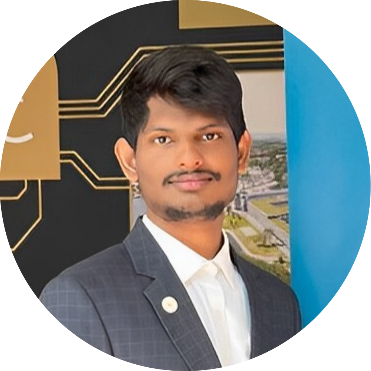
\includegraphics[width=2.7cm,clip]{images/resume_pic_m.png}}
}
\parbox{\dimexpr\linewidth-3.8cm\relax}{
\vspace{-20pt}
\begin{tabularx}{\linewidth}{L r} \\
    {\Huge \scshape  Venkata Sai Yakkshit Reddy Asodi}~
    \href{https://www.cedzlabs.com/yakkshit}{\vspace{1pt}}\\
      India. \\ \vspace{1pt}
     \small \raisebox{-0.1\height}\faPhone\ +91 9493006444 ~ \href{mailto:saiyakkshit2001@gmail.com}{\raisebox{-0.2\height}\faEnvelope\  {saiyakkshit2001@gmail.com}} ~ 
    \href{https://linkedin.com/in/yakkshit/}{\raisebox{-0.2\height}\faLinkedin\ {yakkshit}}  ~
    \href{https://yakkshit.com/}{\raisebox{-0.2\height}\faGlobe\ {yakkshit.com}}  ~
    \href{https://github.com/yakkshit}{\raisebox{-0.2\height}\faGithub{ yakkshit}}
    \vspace{-8pt}
\end{tabularx}
}
\end{center}

\vspace{-23pt}
\section{Summary \faLink}
Full Stack Engineer with expertise in Java, PLSQL, React, and Spring Boot, specializing in developing healthcare technology solutions. Proven track record in implementing CICD pipelines and working with AI/ML technologies. Passionate about creating scalable applications that improve healthcare outcomes and advance health equity through technology. Strong background in Agile methodologies and collaborative development.

\section{\href{https://www.linkedin.com/in/yakkshit/details/skills/}{Technical Skills} \faLink}
\begin{itemize}[leftmargin=0.15in, label={}]
\small{\item{
\textbf{Languages - }{Java, PLSQL, JavaScript (ES6+), Python, HTML5, CSS3} \\
\textbf{Frameworks - }{Spring Boot, React, Drools, Meteor, Vue.js} \\
\textbf{Tools - }{Git, GitHub, Jenkins, Docker, Kubernetes, Postman, Swagger} \\
\textbf{Cloud \& DevOps - }{AWS, Azure, CICD Pipeline Implementation} \\
\textbf{AI/ML - }{Machine Learning, RAG, LLMs, Azure AI}
}}
\end{itemize}
\vspace{-10pt}

\section{Experience \faLinkedin}
\resumeSubHeadingListStart

\resumeSubheading
{\large Circleup AG \faBuilding}{December 2023 -- July 2024}
{Lead Full Stack Engineer}{\faMapMarker \hspace{0.1cm} Zurich, Switzerland}\\
\vspace{10pt}
\textbf{Responsibilities:}
\resumeItemListStart
\vspace{-10pt}
\resumeItem{Architected and developed full-stack applications using Java, Spring Boot, and React, implementing robust CICD pipelines for automated testing and deployment. Integrated AI/ML capabilities to enhance application intelligence and user experience.}
\resumeItem{Led Agile development teams, conducted code reviews, and maintained high code quality standards through automated testing and documentation. Implemented Drools rule engine for business logic management.}
\resumeItemListEnd
\vspace{-3pt}
\textbf{Environment:}\emph{Java, Spring Boot, React, PLSQL, Drools, Jenkins, Git, Agile}

\resumeSubheading
{Cedzlabs \faBuilding}{March 2023 -- July 2024}
{Full Stack Developer}{\faMapMarker \hspace{0.1cm} India}\\
\vspace{10pt}
\textbf{Responsibilities:}
\vspace{-10pt}
\resumeItemListStart
\resumeItem{Developed and maintained healthcare applications using Java and PLSQL, ensuring HIPAA compliance and data security. Implemented React frontend components and integrated with RESTful APIs.}
\resumeItemListEnd
\vspace{-3pt}
\textbf{Environment:}\emph{Java, PLSQL, React, Spring Boot, Git, Agile}

\resumeItem{\textbf{\href{https://linkedin.com/in/yakkshit}{View additional experience on LinkedIn}}}
\vspace{-5pt}

\resumeItem{\textbf{\href{https://linkedin.com/in/yakkshit}{Checkout my other experiences by clicking here}}}
\vspace{-5pt}

\section{Projects \faGithub}
\vspace{-5pt}
\resumeSubHeadingListStart
\resumeProjectHeading
{\textbf{\href{https://ui.cedzlabs.com/resume}{Healthcare Data Analytics Platform}} $|$ \emph{Java, Spring Boot, React, PLSQL}}{2024}\\
\vspace{6pt}
\textbf{Description:}
\vspace{-5pt}
\resumeItemListStart
\resumeItem{Developed a comprehensive healthcare analytics platform using Java Spring Boot backend and React frontend. Implemented PLSQL procedures for efficient data processing and Drools rules engine for complex business logic. Established CICD pipeline using Jenkins for automated testing and deployment.}
\resumeItemListEnd
\vspace{4pt}
\textbf{Tools:}\emph{Java, Spring Boot, React, PLSQL, Drools, Jenkins, Git}
\vspace{-10pt}

\resumeProjectHeading
{\textbf{AI-Powered Health Monitoring System} $|$ \emph{Spring Boot, React, AI/ML}}{2023}\\
\vspace{6pt}
\textbf{Description:}
\vspace{-5pt}
\resumeItemListStart
\resumeItem{Built a health monitoring system integrating AI/ML capabilities for predictive analytics. Implemented using Spring Boot microservices architecture and React frontend, with comprehensive CICD pipeline implementation.}
\resumeItemListEnd
\vspace{4pt}
\textbf{Tools:}\emph{Spring Boot, React, AI/ML, Docker, Kubernetes}
\vspace{-12pt}

\section{Achievements / Certifications}
\resumeSubHeadingListStart
\resumeItemListStart
\resumeItem{Oracle Certified Professional, Java SE Developer}
\resumeItem{AWS Certified Developer - Associate}
\resumeItem{Contributed to open-source healthcare technology projects}
\resumeItem{Led successful implementation of CICD pipelines reducing deployment time by 60\%}
\resumeItemListEnd

\resumeSubHeadingListEnd
\textbf{Strengths:}\emph{Technical Leadership, Problem-solving, Agile Methodologies, Healthcare Domain Knowledge} \\
\textbf{Languages:}\emph{Telugu - Native $|$ English - Fluent $|$ Hindi - Fluent $|$ German - Elementary $|$ Swedish - Elementary}

\vspace{10pt}
\end{document}